\documentclass[12pt]{article}
\usepackage{graphicx}
\usepackage{amsfonts}
\usepackage{amssymb}
\usepackage{mathrsfs}
\usepackage{amsmath}
\usepackage{algorithm2e}
\usepackage{float}
\usepackage[caption = false]{subfig}
\SetKwInOut{Parameter}{parameter}

\usepackage{enumitem}
\textheight 225mm
\textwidth 166mm
\oddsidemargin 0mm
\evensidemargin 0mm
\topmargin -14mm
\parindent 20pt
\pagestyle{plain}
\pagenumbering{arabic}
\renewcommand{\baselinestretch}{1.18}

\usepackage[unicode]{hyperref}
%\usepackage[numbers,sort&compress]{natbib}
\usepackage{booktabs}
% With this package you can set the size of the margins manually:
\usepackage[margin=1in]{geometry}
\usepackage{amssymb}

%\newenvironment{claim}[1]{\par\noindent\underline{Claim:}\space#1}{}
%\newenvironment{claimproof}[1]{\par\noindent\underline{Proof:}\space#1}{\hfill $\blacksquare$}
\usepackage[hyperref,amsmath, thmmarks]{ntheorem}
\usepackage{mathtools}
\DeclarePairedDelimiter\ceil{\lceil}{\rceil}
\DeclarePairedDelimiter\floor{\lfloor}{\rfloor}

\newtheorem{claim}{Claim}
\theoremsymbol{\rule{1ex}{1ex}}
\newtheorem{proof}{Proof}
\theoremsymbol{\rule{1ex}{1ex}}
\newtheorem{claimproof}{Proof of claim}
\title{Planning based on Vonoroi graph and visibility graph}

\author{Yuhao Zhang}

\date{\today}
\begin{document}
\maketitle
% Enter the exercise number, your name and date here:
%\noindent\parbox{\linewidth}{
% \parbox{.25\linewidth}{ \large HW2 }\hfill
% \parbox{.5\linewidth}{\begin{center} \large Yuhao Zhang \end{center}}\hfill
% \parbox{.2\linewidth}{\begin{flushright} \large Jan 22, 2018 \end{flushright}}
%}
%\noindent\rule{\linewidth}{2pt}


%\section{Introduction}
%
%Briefly introduce the problem here. Describe what you have to do and what the goal is. Make sure to cite any references that you might use \cite{knuth}.
\section{Introduction}
The project is an implementation of EKF-SLAM on Sunfounder's PiCar-V platform and a webcam attached to it is used. With the help of QR codes as landmarks, the webcam is turned into a distance-bearing sensor.
\section{Planning based on Vonoroi graph and visibility graph}
In this project the EKF-SLAM system will be built from scratch. For a thorough introduction to EKF-SLAM, please check \cite{ekf}. In this project, the landmarks used for SLAM will be QR markers. The SLAM will only consider 2D-plane, therefore the landmarks will be abstracted as points on the plane, although theoretically the QR markers can be used as a 3D object that enables more information and features to be extracted. The detail will be discussed in Sec. {\ref{PnP}}.
\label{EKF}
\section{Localization}
One major problem for Sunfounder's PiCar-V platform is the lack of a distance-bearing sensor that would make localization with landmarks much easier. However, with the help of known-sized QR tags as 3D object, it is plausible to convert a plain webcam into a distance-bearing sensor.
\subsection{Distance and Pose estimation using PnP}
\label{PnP}
\label{pose}
With a simple pinhole model the scene view $s$ of a camera is formulated as:
$$
s
\begin{pmatrix}
u \\
v \\
1 \\
\end{pmatrix}
=
\begin{pmatrix}
f_x & 0 & c_x \\
0  & f_y &c_y \\
0 & 0 & 1\\
\end{pmatrix}
\begin{pmatrix}
r_{11} & r_{12} & r_{13} & t_1\\
r_{21}  & r_{22} &c_{23} & t_2\\
r_{31} & r_{32} & r_{33} & t_3\\
\end{pmatrix}
\begin{pmatrix}
X \\
Y\\
Z \\
1\\
\end{pmatrix},
$$
where $(X,Y,Z)$ is the coordinate of the object point in world reference frame, $(u,v)$ is the coordinates of the projected object on the view. The first factor on the right hand side is the camera matrix which depicts the intrinsic properties of the camera, while the second factor is the rotation-translation matrix that transforms from world reference frame to the camera frame.

The rotation-translation matrix $R-T$ is solvable by first, detecting the QR code using library such as \texttt{zbar}. Second,  finding the corner points of it and associate with their projections on the view. Once $R-T$ is obtained, one can solve directly for its inverse, as the inverse serves directly for pose estimation of the camera. 

Given $R$ which is the rotation matrix, the inverse of it is denoted as $R^{-1}=R^{T}$. Then the coordinates of the camera in world reference frame are obtained as 

$$(x,y,z)=-R^T V.$$
And the distance between the camera and the object:

$$d=\sqrt{(X-x)^2+(Y-y)^2+Z-z)^2}.$$
Furthermore, the Euler angles representation can also be acquired easily form $R$. As for car-like mobile robots, the motion is usually confined to 2-D plane. Consider such a plane is depicted is a right-hand coordinate system as $x-z$ plane and axis $y$ is pointing to the ground.  Then only Euler angle $ \theta_y$ is of interest. Then the problem can be largely simplified.  For a landmark $M(X,Y,\gamma)$ in world reference frame, the current pose of the camera is 

$$(X-d\cos(\theta_y),Y+d\sin(\theta_y),\pi/2-\theta_y+\gamma).$$
\subsection{Bearing}
The bearing of the object with respect to the camera can be calculated directly using the rotation-translation matrix $R-T$. But in the experiments such calculation turns out to be quite inaccurate and is not sufficient for real application. Therefore in the rest of the paper the bearing is obtained as $$(c_x-c_c)\times \frac{d}{f_x},$$

where $c_x$ is the $x$ principle point as shown in the camera matrix, $c_c$ is the center of the QR tag in camera frame and $f_x$ is the $x-$direction focal length of the camera.

With this pose estimation, one can combine a control algorithm with feedback from QR codes detected by camera.

A picture showing the performance of such model is plotted as  Fig. (\ref{QR}).
\begin{figure}[htbp]
\centering
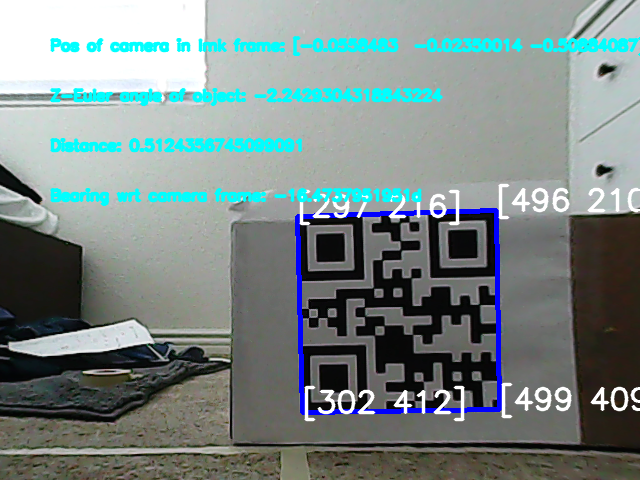
\includegraphics[width=0.7\textwidth]{../figures/bearing_distance.png}
\caption{The QR code used as a landmark.}\label{QR}
\end{figure}
\section{Kinematics and control law}
\label{kine}
The kinematics of the car is orthogonal to the current 
Ackerman model can be used to describe the kinematics of a car-like robot: 
$$\frac{d x}{dt}=v\cos \theta,$$
$$\frac{d y}{dt}=v\cos \theta,$$
$$\frac{d \theta}{dt}=\frac{v}{L}\tan \gamma,$$
where $(x,y)$ is the position of the middle point of the back wheel axis of the robot in world reference frame. $\theta$ is the angle of pose of the robot. The steering wheel angle is $\gamma$ and the velocity of the back wheel is $v$. $L$ is the length of the vehicle or wheel base.

These equations can be re-written as:
$$
\begin{pmatrix}
\frac{d x}{dt} \\
\frac{d \omega}{dt} \\
\frac{d \theta}{dt} \\
\end{pmatrix}
=
\begin{pmatrix}
\cos \theta & 0 \\
\sin \theta & 0 \\
0 & 1\\
\end{pmatrix}
\begin{pmatrix}
v \\
\omega
\end{pmatrix}.
$$
With the initial position-pose $(x,y,\theta)$ and the goal $(x^*,y^*,\theta^*)$, it is more convenient to write the equations in polar system via a transformation:
$$\rho=\sqrt{\Delta_x^2+\Delta_y^2},$$
$$\alpha=\arctan \frac{\Delta_y}{\Delta_x}-\theta,$$
$$\beta=-\theta-\alpha+\theta^*.$$

The linear control law for $-\pi/2<\alpha\le \pi/2$, i.e. the waypoint is in front of the vehicle is:
$$v=k_\rho \rho,$$
$$\omega=k_\alpha \alpha+k_\beta \beta,$$
where $k_\rho$, $k_\alpha$, $k_\beta$ are arbitrary coefficients that satisfies $k_\rho>0, k_\beta<0,k_\alpha-k_\rho>0.$

The control law for the cases where the waypoint is behind the vehicle is the same as above, but with transformed angles:

$$\alpha'=-\pi-\beta,$$
$$\beta'=-\pi-\alpha,$$
and $v'=-v$.

%\section{Pose estimation}
%\label{pose}
%Without the feedback from sensors, it is required to estimate the motion from the kinematics of the robot directly. Using the linear approximation of the kinematics equations for a short time period $\Delta t$ one can obtain
%$$\Delta(x,y,\theta)=(v\cos \theta \Delta t ,v \sin \theta \Delta t, v/L \tan \gamma \Delta t).$$
%
%Alternatively, the exact solution can be obtained by solving these differential equations directly:
%$$\Delta(x,y,\theta)=(R_b\sin(K\Delta t),R_b(1-\cos(K\Delta t)),K\Delta t),$$
%where $R_b=L/\tan \gamma$ and $K=v/R_b$. However, this estimation is non-linear and makes the control law purposed unstable. Therefore the linear approximation will be used in the following sections.


\section{implementation and setup}

The EKF-SLAM algorithm purposed in Sec.(\ref{EKF}) is implemented in library \texttt{EKF\_SLAM.py} following and being translated from the Matlab code provided in \cite{ekf}. The pose estimation algorithm purposed in Sec.(\ref{pose}) has been implemented in library \texttt{QRDB.py}.  Additionally, a script that calls these libraries is provided as \texttt{EKF-SLAM-QR-DB.ipynb}. 

After initialization, the algorithm is time sampled every $0.5$ seconds and at each step, the camera takes 20 images and runs QR code detection on them. All vision data is precessed for un-distortion. Then the average of the results are taken. The control signal is a constant to enforce the robot moves in circle. The algorithm utilizes the $R-T$ matrix described in Sec.(\ref{pose}) to localize the camera in world frame based on the QR codes scanned.  Finally the EKF-SLAM module will be called to apply Kalman filter on the observations.


%\begin{figure}[htbp]
%\centering
%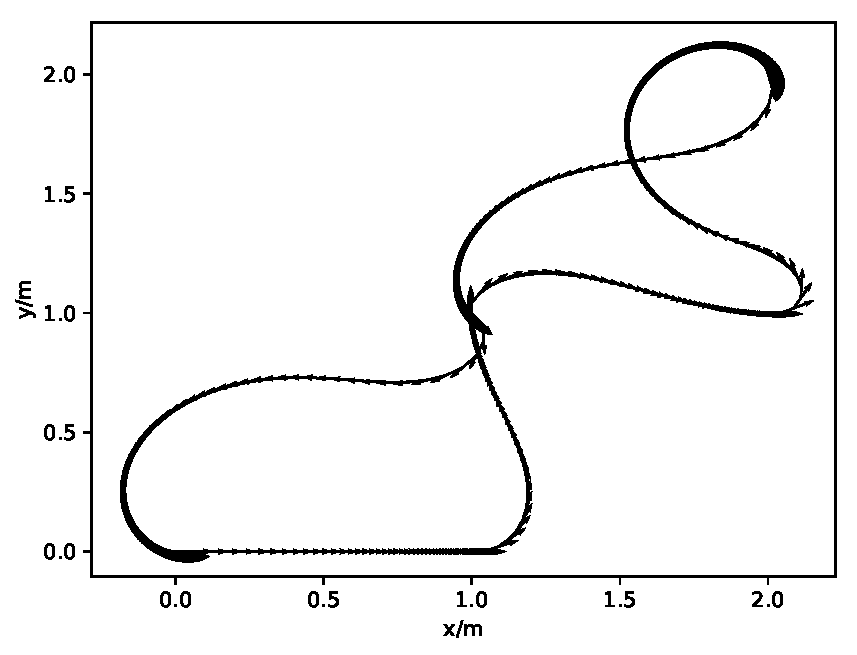
\includegraphics[width=0.7\textwidth]{../ideal_traj.pdf}
%\caption{One generated trajectory.}\label{ideal}
%\end{figure}
\section{Experiment and conclusion}
The algorithm is run on Sunfounder's PiCar-V platform with the setup map shown as Fig.(\ref{setup}).  The actual photo of the test ground is shown as Fig.{\ref{ph}}.
\begin{figure}[htbp]
\centering
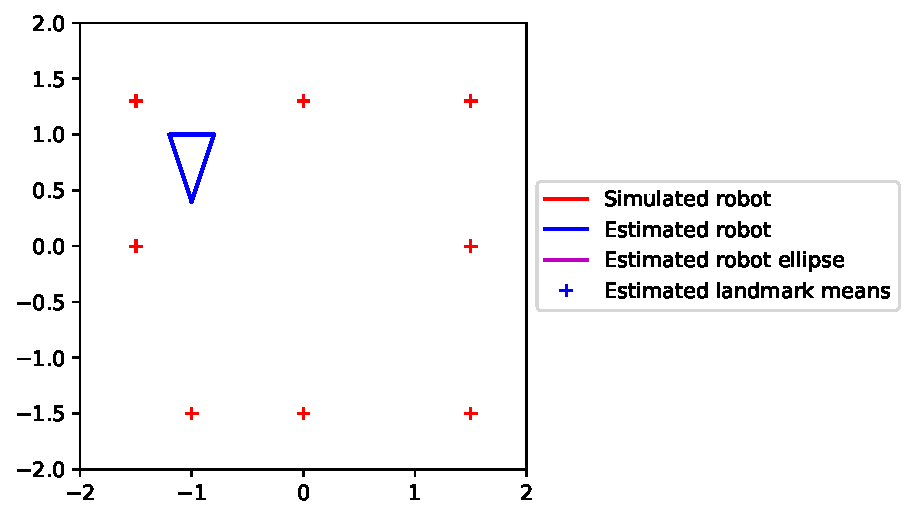
\includegraphics[width=0.7\textwidth]{./figs/20180514-044756/setup.pdf}
\caption{The initial map and the initial pose of the robot. Data entry denoted as \textit{Simulated} means the optimal situation and \textit{Estimated} means the actual data feedback from the sensor and processed with Kalman filter.}\label{setup}
\end{figure}
\begin{figure}[htbp]
\centering
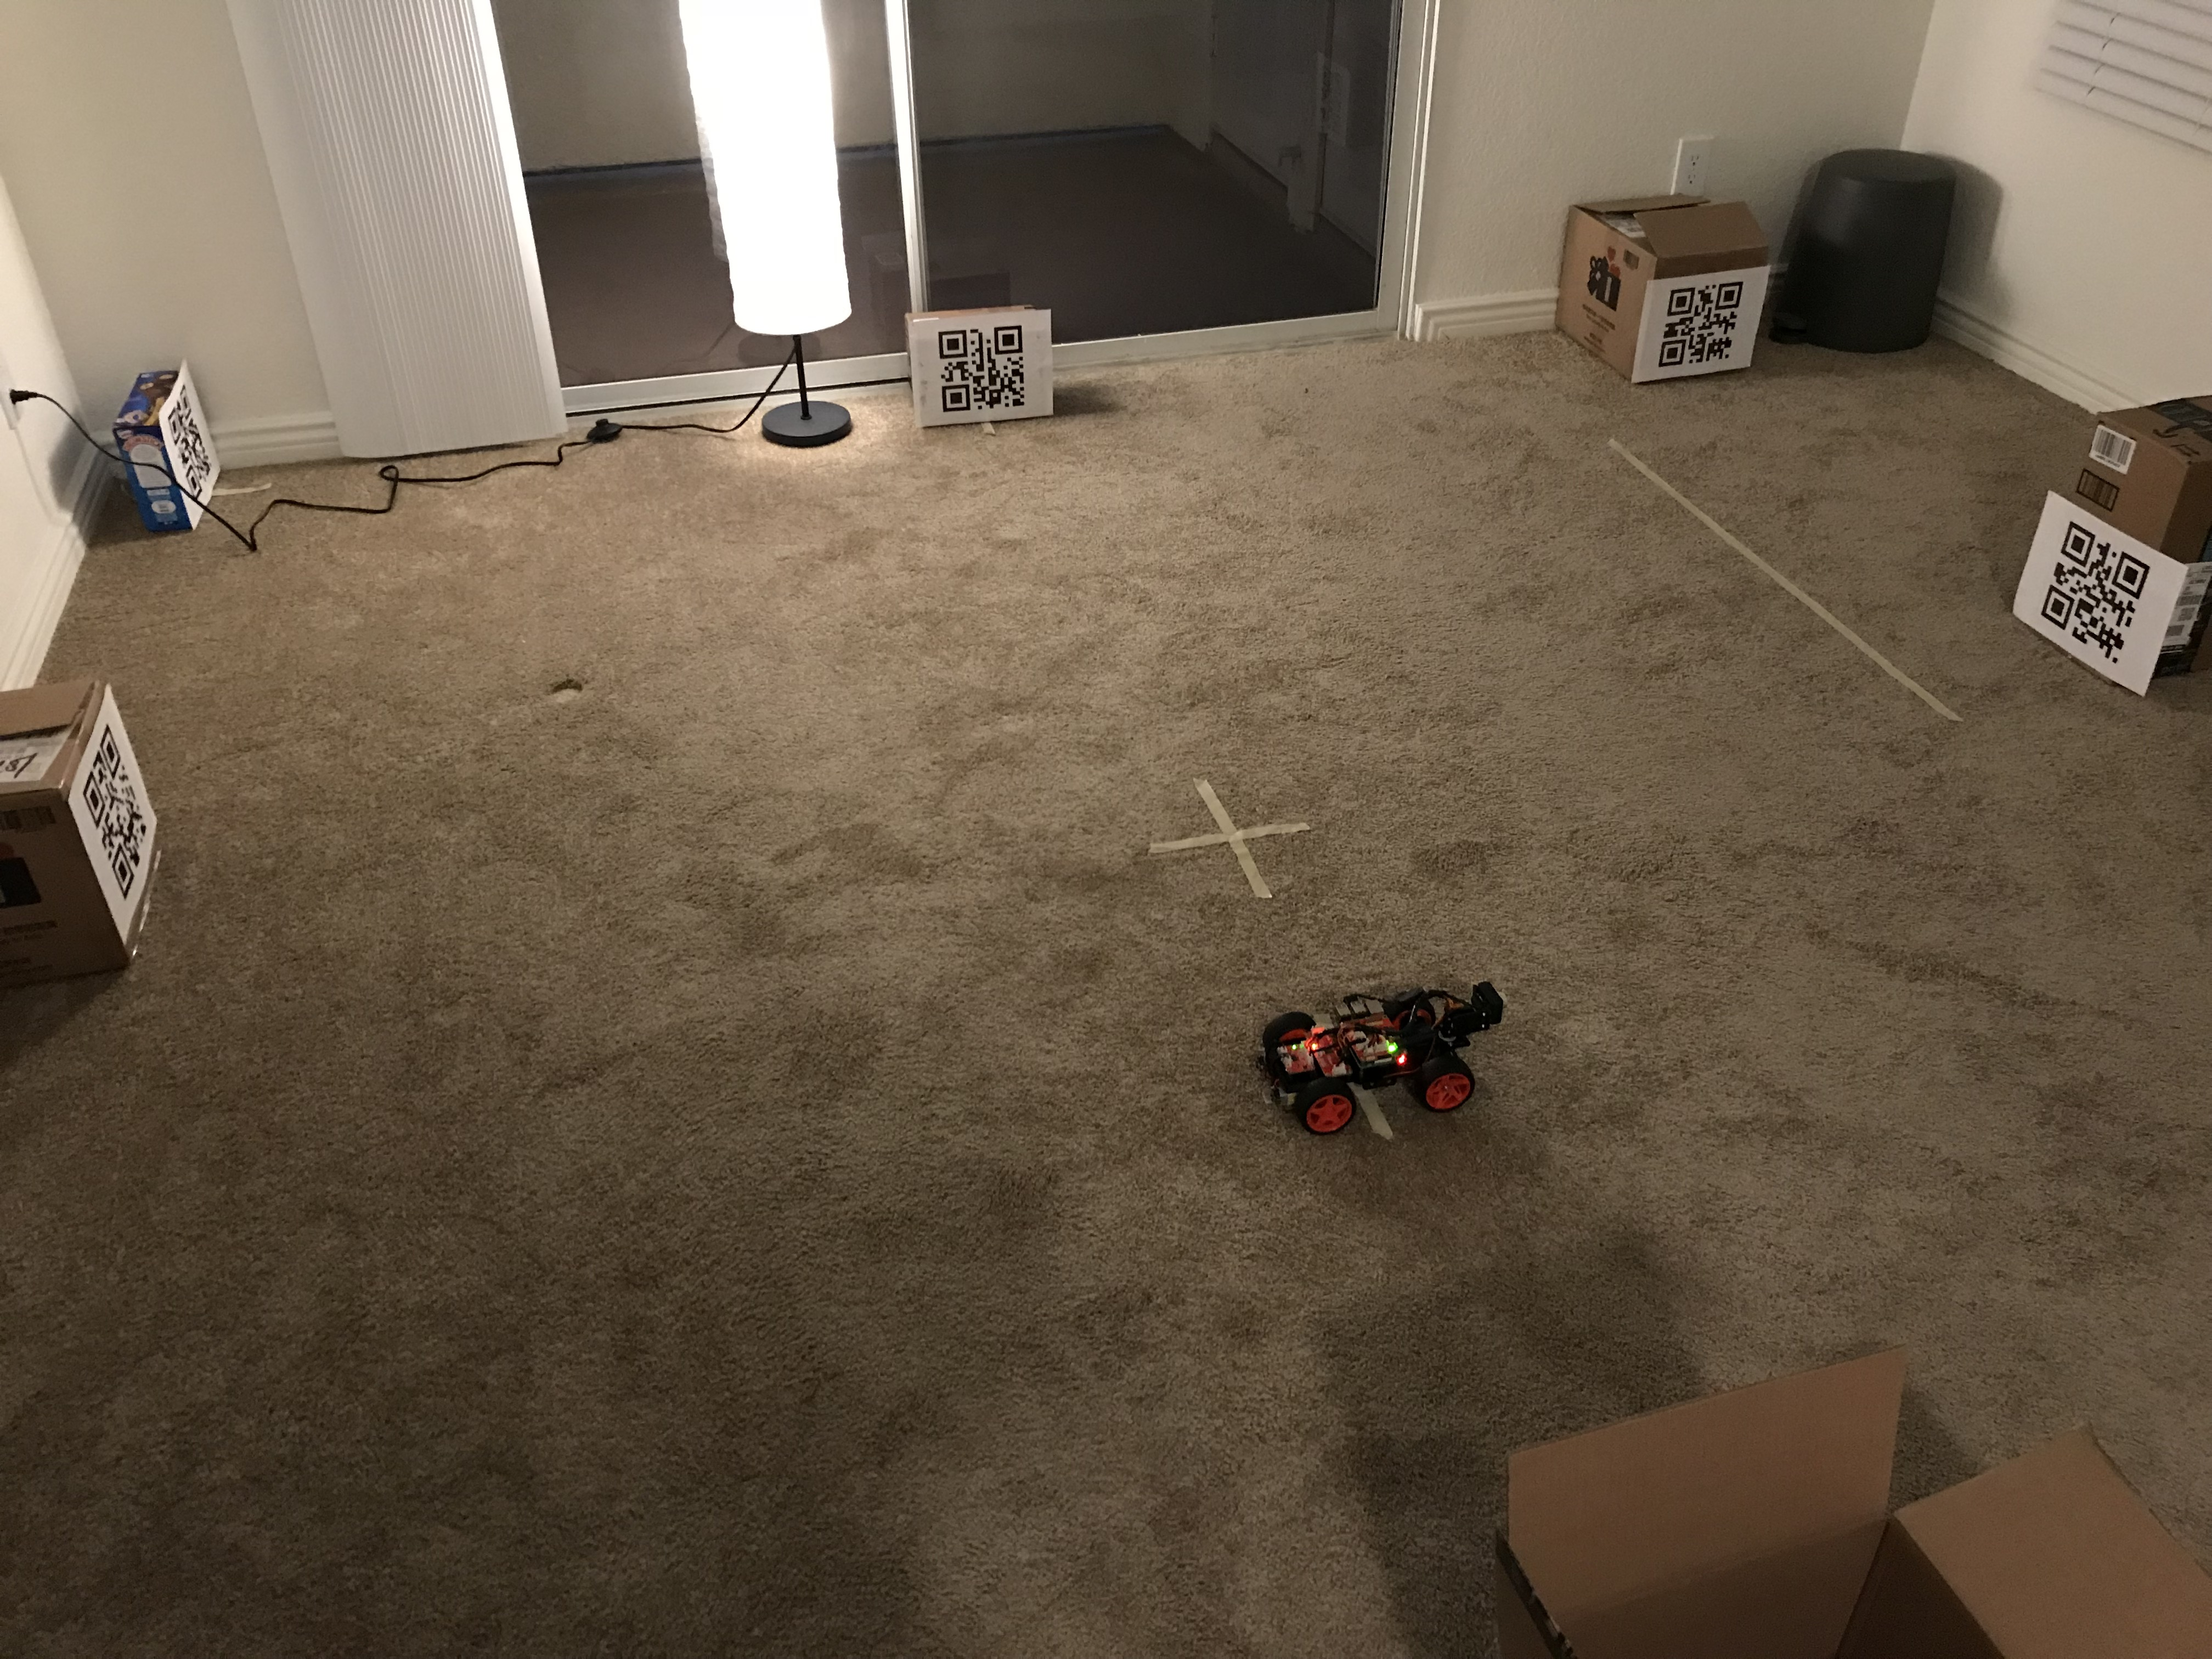
\includegraphics[width=0.5\textwidth]{./figs/pg.JPG}
\caption{The actual photo of the test ground. }\label{ph}
\end{figure}
The landmarks are cardboards with QR tags attached to. 

Some intermediate results are shown as Fig.{\ref{some}}. It can be seen that the accuracy(distances between means of estimated landmarks and their true position) grows steadily as the robot drives multiple times around the test ground. Also the standard deviations of the estimations (the eclipses of the estimated landmarks) drops drastically as the drive goes on.


\begin{figure}[h]
\subfloat[step 1]{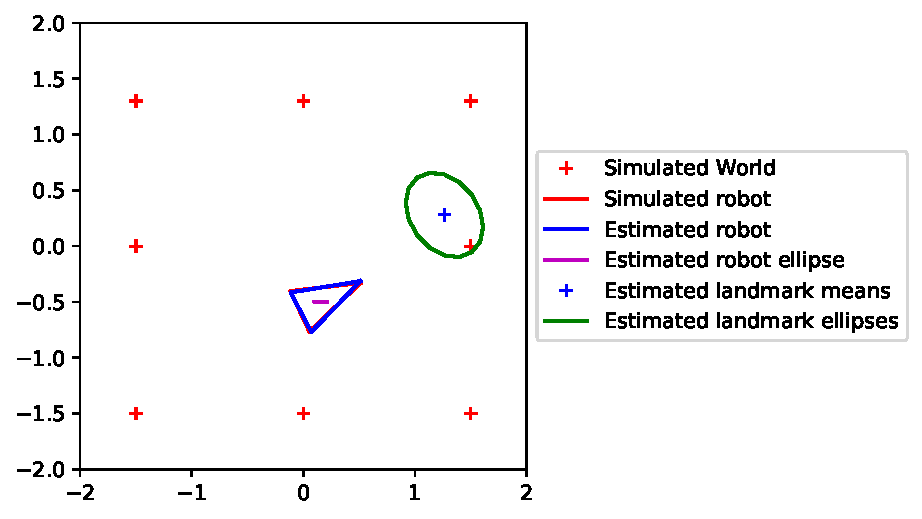
\includegraphics[width = 3in]{./figs/20180514-044756/0.pdf}} 
\subfloat[step 5]{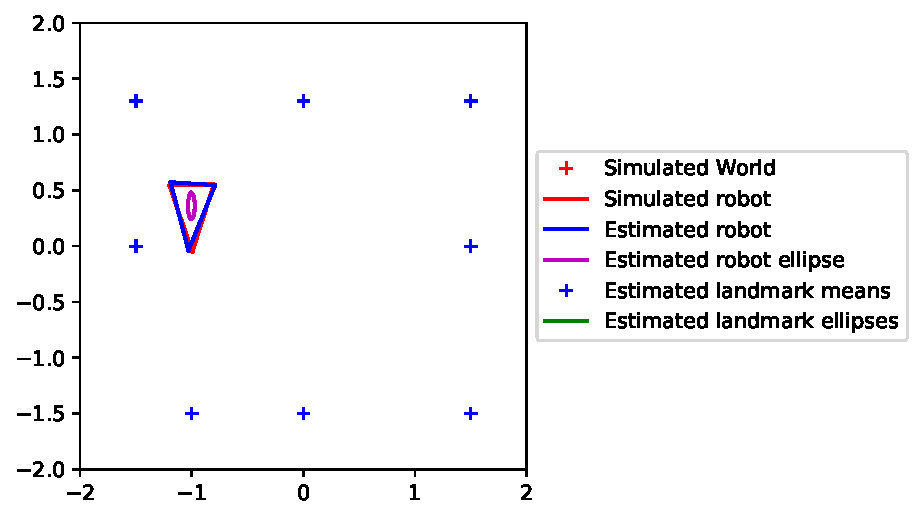
\includegraphics[width = 3in]{./figs/20180514-044756/5.pdf}}\\
\subfloat[step 10]{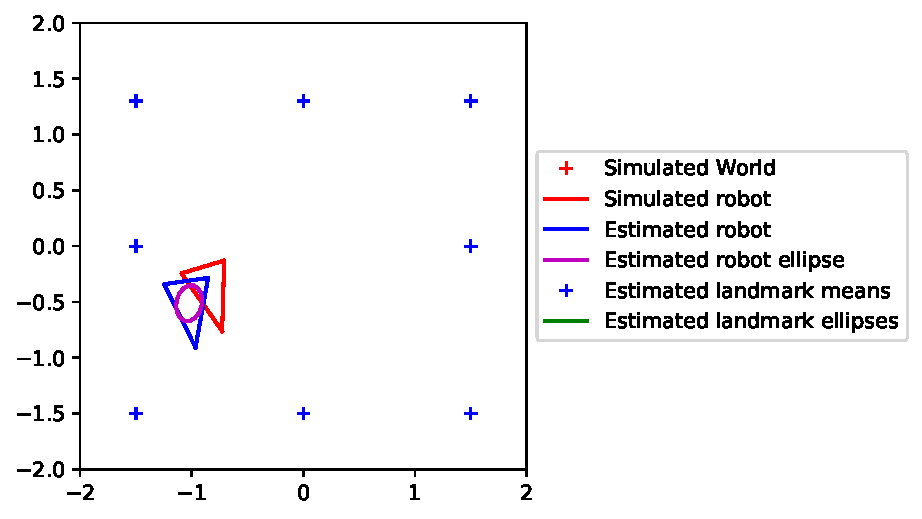
\includegraphics[width = 3in]{./figs/20180514-044756/10.pdf}}
\subfloat[step 15]{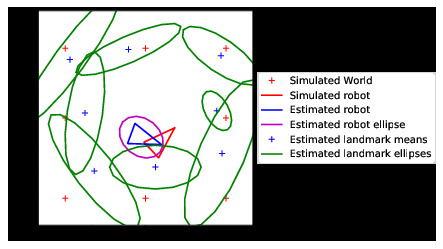
\includegraphics[width = 3in]{./figs/20180514-044756/15.pdf}} \\
\subfloat[step 20]{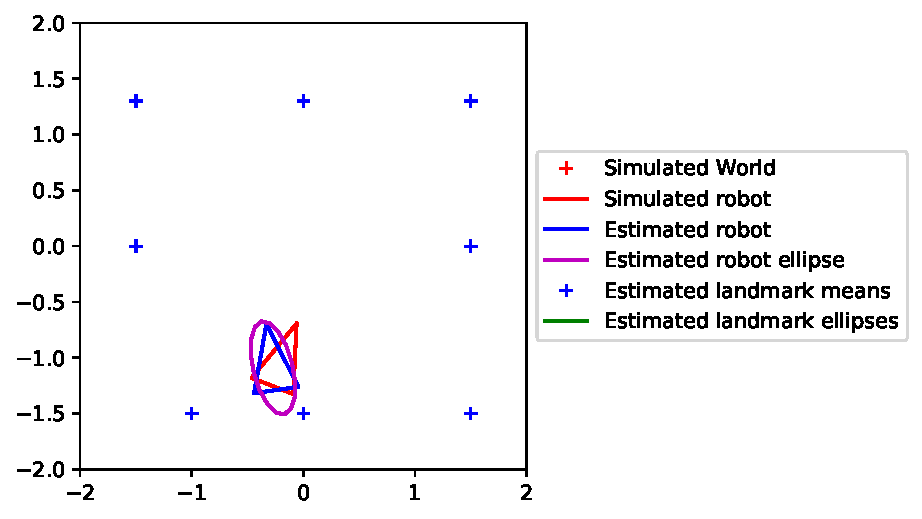
\includegraphics[width = 3in]{./figs/20180514-044756/20.pdf}} 
\subfloat[step 30]{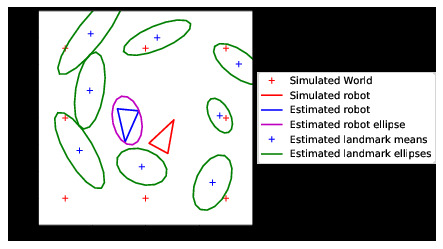
\includegraphics[width = 3in]{./figs/20180514-044756/30.pdf}} \\
\subfloat[step 50]{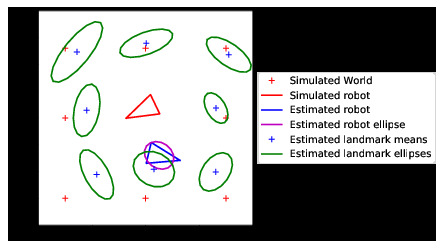
\includegraphics[width = 3in]{./figs/20180514-044756/50.pdf}} 
\subfloat[step 145]{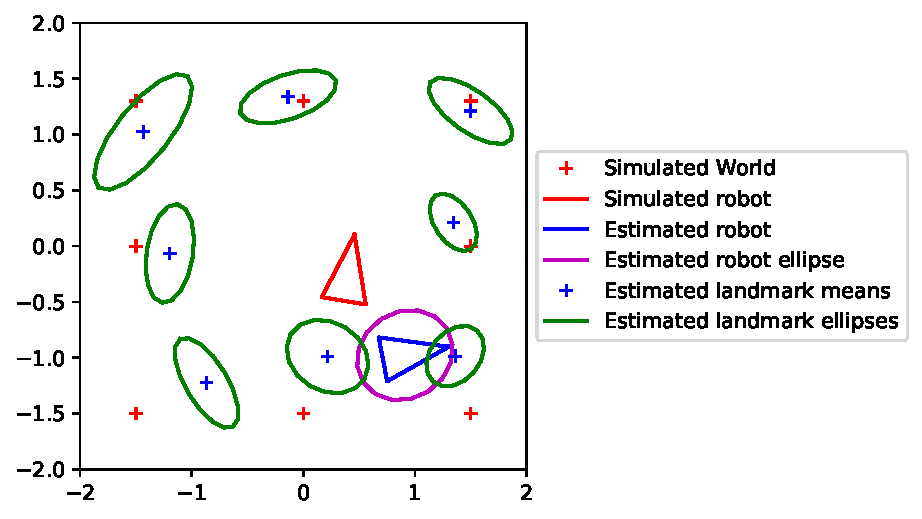
\includegraphics[width = 3in]{./figs/20180514-044756/145.pdf}} \\
\caption{Intermediate maps as EKF-SLAM goes on. Data entry denoted as \textit{Simulated} means the optimal situation and \textit{Estimated} means the actual data feedback from the sensor and processed with Kalman filter.}
\label{some}
\end{figure}


%To see the results of the full run, please check \texttt{ani.gif}.

Given that PiCar-V's price and the mediocre performance of the webcam equipped, the results are promising. The final map still has some deviation from the estimated map, which might be due to the error of placement of the landmarks. 

The algorithm of this experiment not only utilizes the coordinates generated by the feedback of QR codes, but also calculates the Euler angles with respect to the rotation-transformation matrix, which means that the orientation of the robot can also be calculated per QR marker scan. But this application is irrelevant to the 2D-EKF-SLAM and the performance on the webcam is poor. The reader might find it useful under other settings.
 

\clearpage
\begin{thebibliography}{9}

\bibitem{ekf} 
Joan Sol\`a: Simulataneous localization and mapping
with the extended Kalman filter, retrieved at 05-13-2018,
\\\texttt{http://www.iri.upc.edu/people/jsola/JoanSola/objectes/...\\curs\_SLAM/SLAM2D/SLAM\%20course.pdf}
\end{thebibliography}


 
\end{document}



%\begin{figure}[htbp]
%\centering
%\includegraphics[width=0.5\textwidth]{./src/lctwomethods.eps}
%\caption{Learning curve for steepest-direction coordinate descent and random-feature coordinate descent.}\label{fig1}
%\end{figure}

%\begin{table}[hp]
%\centering
%\caption{Experiment results}
%\label{tab1}
%\begin{tabular}{llr}
%
%$M$    & Prototype & Error rate (\%) \\
%\hline
%1000      & random    & $13.02 \pm  0.73$    \\
%          & random*        & $11. 84 \pm 0.20$      \\
%5000       & random     & $6.63 \pm 0.11$      \\
%		& random*     &$6.42 \pm 0.22$      \\
%10000       & random     & $5.07 \pm 0.2$     \\
%		 & random*      & $4.8 \pm 0.26$       \\
%\hline
%\end{tabular}
%\end{table}







%\subsection{Task 3}
%For 1000 different 100$\times$100 lattices with different $p$ values, the shortest path and the life time of fire is plotted in Fig.(\ref{fig3}). It can be seen clearly that the curves have a phase change point at $p_c\approx0.59$, after which the minimal step and life of fire drop quickly and approximates 100, the width of lattice.
%
%\begin{figure}[htbp]
%\centering
%\includegraphics[width=0.5\textwidth]{../figures/N100pvariable.eps}
%\caption{1000 different 100$\times$100 lattices with different $p$ values, the shortest path and the life time of fire}\label{fig3}
%\end{figure}
%
%For different values of width of lattice $N$, we use 1000 different random lattices per $N$ to find the correlation between the ratio of spanning cluster and the $p$ value, which is plotted in Fig.(\ref{fig4})
%
%
%\begin{figure}[htbp]
%\centering
%\includegraphics[width=0.5\textwidth]{../figures/ratio.eps}
%\caption{1000 different lattices of $N=50, 100, 200$ with different $p$ values, the ratio of the spanning cluster}\label{fig4}
%\end{figure}
%
%
%\section{Discussion}
%It can be found through these figures that $p_c\approx0.59$ and it is irrelevant to the width of lattice $N$.
%\begin{thebibliography}{99}
%
%\bibitem{knuth}
%  Knuth, Ervin D.,
%  \emph{The art of computer programming}, 
%  Addison Wesley, Massachusetts,
%  3rd edition,
%  1997.
%
%\end{thebibliography}

\end{document}